%************************************************
\chapter{Conformal Field Theory}\label{ch:Conformal Field Theory}
\minitoc\mtcskip
%************************************************

\noindent Conformal field theories may in general be regarded as  
quantum field theories whose symmetry group is the conformal group,
namely the group of angles preserving transformations of the space-time
(see definition below in \ref{Conformal transformations}).
Motivations to investigate such a mathematical structure lie
in many different models appearing in nature: physical 
realisations can be found, for example, in the free
Maxwell theory, the massless Dirac field in 4-dim, not to 
mention the whole construction of string theory and all the 
related areas, as well as applied models in material sciences and
engineering. A very interesting class of models, and in
particular the actual models we shall be looking at, occurs 
in two-dimensional theories which are chirally invariant: 
in this case the observables depend on the so-called 
``light-cone'' variables $x_{\pm}\coloneqq x^0\pm x^1$ only as
\[
\phi(x^0,x^1)=\phi^+(x^+)\otimes \bm{1}^- \pm \bm{1}^+\otimes 
\phi^-(x^-)
\]
and the set of observables $\alg{O}=\alg{I}\otimes
\alg{J}\subset\mathcal{B}(O)$ can be decomposed into
their respective chiral parts, $\alg{I}$ and $\alg{J}$,
with $O$ given by $O=I\times J$. 
Two independent one-dimensional copies 
living on the light rays $x_{\pm}\in\R$ are therefore obtained
and the entire theory can be reconstructed by taking back
the tensor product. The real line where each of the variables
$x_{\pm}$ lives can be compactified on the circle $\s$ via the
Cayley transform 
\begin{center}
 \begin{minipage}{.48\textwidth}
 \begin{align*}
 \textrm{C}\colon &\R\to\s\setminus\set{-1}\\
 & x\mapsto z=\frac{1+ix}{1-ix}
 \end{align*}
 \end{minipage}
 \begin{minipage}{.48\textwidth}
 \centering
 \def\radius{0.8}
 \begin{tikzpicture}[scale=1]
 \path (0,0) coordinate (O);
 \path (\radius,0) coordinate (A);
 \path (-\radius,0) coordinate (B);
 \path (\radius,0.4) coordinate (R);
 \path (\radius,0.85) coordinate (S);
 \path (0.85,0.4) coordinate (U);
 \path (0.85, 0.85) coordinate (V);
 \draw (O) circle (\radius);
 \draw [->] (\radius,-1.2) -- (\radius,1.5) node[right] {\scriptsize{$\mathbb{R}$}};
 % axis ------
 \draw [->][style=dotted](-1,0) -- (1.2,0) node[below] {\tiny{${x}$}}; %x-axis
 \draw [->][style=dotted](0,-1) -- (0,1.2) node[left] {\tiny{${y}$}}; %x-axis
 % ------
 \path (28:0.85) coordinate (P);
 \path (53:1.05) coordinate (Q);
 % arcs ------
 \draw [line width=0.3mm,color=navy!60!](P) arc (28:50:1);
 % lines ------
 \draw (B) -- (R);
 \draw (B) -- (S);
 \draw [line width=0.3mm,color=navy!60!](U) --(V);
 % circle in -1 ------
 \draw (-0.8,0)[fill=white] circle (0.07);
 \end{tikzpicture}
 \end{minipage}
\end{center}
after identifying $\textrm{C}^{-1}(\s)\equiv\overline{\R}=\R
\cup\set{\infty}$. This allows us to look at theories defined 
on the circle, from which two-dimensional chirally invariant
field theories can be reconstructed by following back the above
procedure. So to speak, in case of chiral conformal field theories,
the space-time is (two copies of) the unit circle whose open intervals
form the set of space-time regions under investigation. In particular,
we shall see that the mutual position of such intervals will carry
causality and all the rest of properties that physics requires to
be fulfilled through mathematical axioms.

The conformal group of the two-dimensional theory 
can be decomposed as $\textrm{Conf}_2=\textrm{Conf}_1\times
\textrm{Conf}_1$, where $\textrm{Conf}_1=\Diff(\s)$ is identified
with the group of the orientation preserving diffeomorphisms 
on the compactified real line (see below).
\begin{example}[Massless Dirac field in two dimensions]
The massless Dirac equation in two dimensions reads
\[
i\slashed{\partial}\,\Psi(x^0,x^1)=0
\]
which can be turned into 
\[
(\partial_0+\partial_1\,\gamma^5)\,\Psi=0
\]
where $\gamma^5=\gamma^0\gamma^1$. By using the chiral 
projection $P_{\pm}=1/2(\bm{1}\pm\gamma^5)$ the Dirac spinor
decouples into $\Psi=P_+\,\Psi_+ + P_-\,\Psi_-$, with 
$\gamma^+,\gamma^-$ eigenvectors of $\gamma^5$ with eigenvalues 
$\pm 1$. Introducing the light cone coordinates $x_{\pm}=x^0\pm x^1$ 
leads to
\[
\partial_{\pm}\,\Psi_{\pm}(x_+,x_-)=0,
\]
thus $\Psi_{\pm}\equiv\Psi_{\pm}(x_{\mp})$, only depending 
on one variable at a time. Therefore the argument introduced
above directly applies.
\end{example}


%*******************************************************
\section{Conformal transformations}
\label{Conformal transformations}
Conformal transformations are maps $f\colon \vN^d\to\vN^d$
preserving angles in the $d$-dimensional Minkowski space-time 
$\vN^d$: this means that the only possible way
the metric may transform is up to a scaling (positive) factor 
$g'_{\mu\nu}(x')=\e^{\omega(x)}g_{\mu\nu}(x)$. 
Working out the definition we are led to the following set of 
transformations (\cite*{KE:1998}):
\begin{table}[htbp]
\caption{Conformal transformations}
\centering
  \begin{tabular}{lll}
  \toprule
  Generator     & transformation     &    \\
  \midrule
  $P_{\mu}$     & translations       &    $x'^{\mu}=x^{\mu}+a^{\mu}$\\
  $M_{\mu \nu}$ & Lorentz            &    $x'^{\mu}=\Lambda^{\mu}_{\phantom{\mu}
                                          \nu}\,x^{\nu},\quad \Lambda\in
                                          \textrm{SO}(p,q)$\\
  $D$           & dilations          &    $x'^{\mu}=\lambda\,x^{\mu},\quad 
                                          \lambda\in\R$\\
  $K_{\mu}$     & special conformal  &    $x'^{\mu}=\frac{x^\mu-b^{\mu}x^2}
                                          {1-2b\cdot x+b^2 x^2}$\,.\\
  \bottomrule                                        
  \end{tabular}
\end{table}

The first two classes generate the Poincar\'{e} group
$\textrm{SO}(p,q)\ltimes\R^d$ and together with the dilations
they generate the Weyl group. In the case $d\neq 2$ the whole
conformal group is $(d+1)(d+2)/2$-dimensional. The generators
obey the following commutation relations, which in turn define 
the conformal algebra \cite*{dFMS:1997}
 \begin{equation}
  \begin{split}
  \comm{D,P_{\mu}}&=i P_{\mu}\\
  \comm{D,K_{\mu}}&=-i K_{\mu}\\
  \comm{K_{\mu},P_{\nu}}&=2i\,(g_{\mu \nu}D-M_{\mu \nu})\\
  \comm{K_{\rho},M_{\mu \nu}}&=i\,(g_{\rho \mu} K_{\nu} -
                              g_{\rho \nu}K_{\mu})\\
  \comm{P_{\rho}, M_{\mu \nu}}&=i\,(g_{\rho \mu} P_{\nu} -
                              g_{\rho \nu}P_{\mu})\\
  \comm{M_{\mu \nu},M_{\rho \sigma}}&=i\, (g_{\nu \rho}M_{\mu \sigma}
                              +g_{\mu \sigma}M_{\nu \rho}-
                              g_{\mu \rho}M_{\nu \sigma}-
                              g_{\nu \sigma}M_{\mu \rho}).
  \end{split}
 \end{equation}




\bigskip
For our purposes we restrict to the two-dimensional case, 
where, interestingly enough, the conditions for a map to be 
conformal reduce to the Cauchy-Riemann equations. In terms of 
complex variables they are holomorphic and anti-holomorphic maps
$z\mapsto f(z),\ \bar{z}\mapsto \bar{f}(\bar{z})$ such that
$\partial_{\bar{z}}f(z)=\partial_{z}\bar{f}(\bar{z})=0$.
When the complex variable corresponds to the Cayley transform
of a lightray coordinate $x_{\pm}$, namely on a compactified
Minkowski space-time $\vN^2=\s\times\s$, then the conformal group
is identified with $\Diff(\s)\times \Diff(\s)$, two commuting
copies of diffeomorphisms of the circle which we are going to
look once at a time.
\begin{example}
Here we show some examples of what simple conformal 
transformations on the plane look like:

\bigskip
\begin{center}
 \begin{figure}[htbp]
 \centering
  \begin{minipage}{.45\textwidth}
  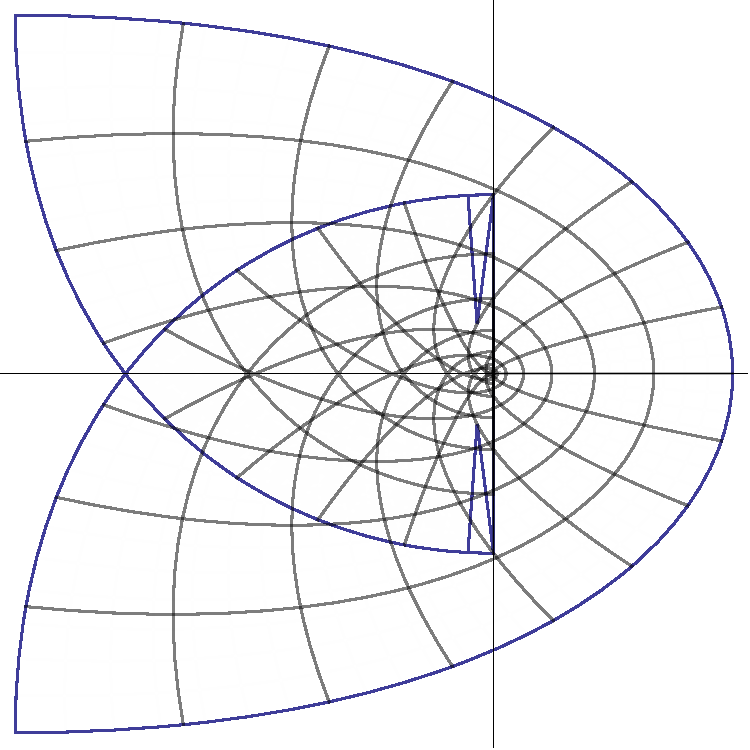
\includegraphics[width=.8\textwidth]{Graphics/conf5.pdf}
  \caption*{$f(z)=z^3$}
  \end{minipage}
  \begin{minipage}{.45\textwidth}
  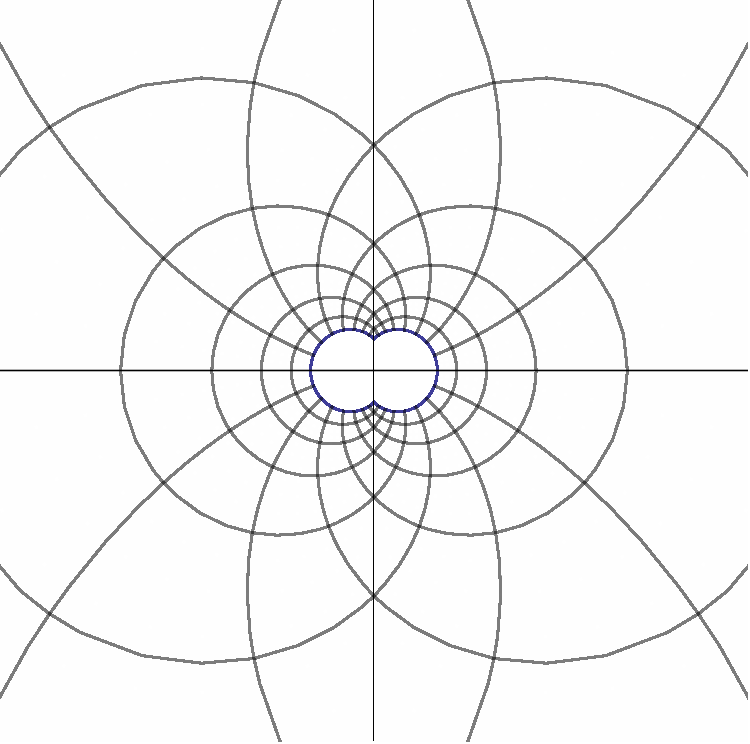
\includegraphics[width=.8\textwidth]{Graphics/conf2.pdf}
  \caption*{$f(z)=1/z^2$}
  \end{minipage}
  
  \bigskip
  \begin{minipage}{.45\textwidth}
  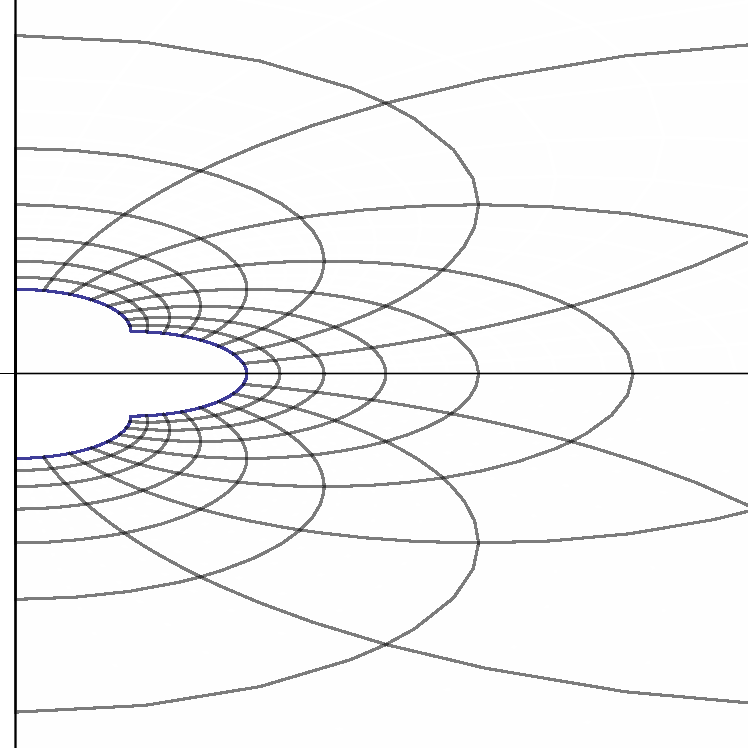
\includegraphics[width=.8\textwidth]{Graphics/conf3.pdf}
  \caption*{$f(z)=1/z$}
  \end{minipage}
  \begin{minipage}{.45\textwidth}
  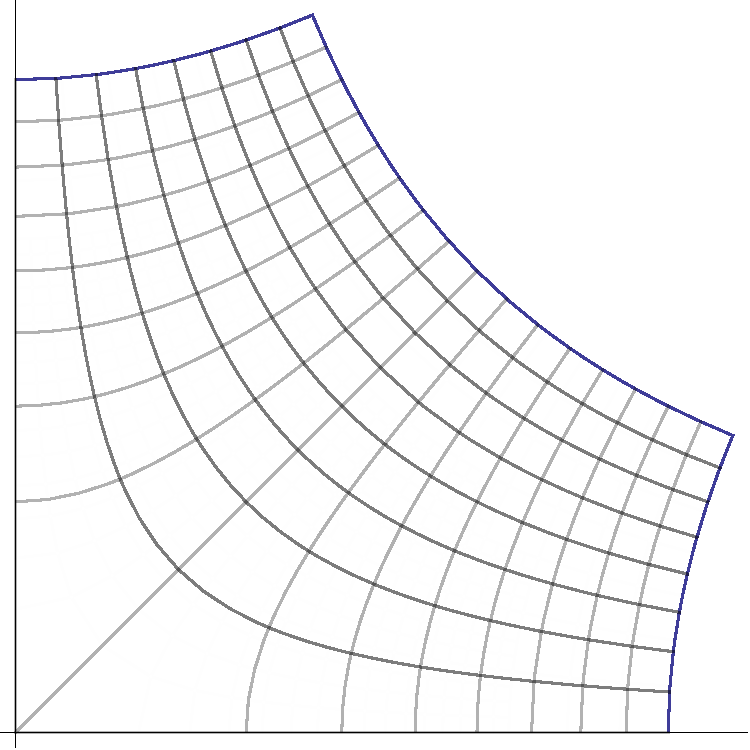
\includegraphics[width=.8\textwidth]{Graphics/conf4.pdf}
  \caption*{$f(z)=\sqrt{z}$}
  \end{minipage}
  \end{figure}
\end{center}
\end{example}
%\pagebreak


%*******************************************************
\section{The Virasoro algebra}
\label{The Virasoro algebra}
Let $\Diff(\s)$ be the group of orientation preserving
diffeomorphisms on $\s$, which in turn coincides with
the conformal transformations leaving the circle invariant. 
Its Lie algebra corresponds to the algebra of smooth
vector fields on the circle whose complexification gives 
rise to the Witt algebra with basis elements $l_n\coloneqq
-z^{n+1} \frac{d}{dz}$, such that
\[
\comm{l_n,l_m}=(n-m)l_{m+n}.
\]
Since we are looking for projective unitary representations of
positive energy we shall be concerned with its unique non-trivial 
central extension (see \cite*{KE:1998}), the Virasoro algebra, 
given in terms of generators $L_n$
\begin{equation}
\label{Vir}
\comm{L_n,L_m}=(n-m)L_{n+m} + \frac{c}{12} m(m^2-1)\,
\delta_{n+m}\bm{1}.
\end{equation}
$L_0$ is referred to as the conformal Hamiltonian and we are interested
in irreducible unitary representations $\pi$ of the above algebra with 
positive energy, namely the spectrum of $L_0$ is required to be positive.
Those representations have been fully classified (see \cite*{FQS})
and are given in terms of pairs $(c,h)$ where $c$ is the central
term appearing in \eqref{Vir} and $h$ is the lowest weight
\[
\pi_{(c,h)}(L_0)\ket{h}=h\ket{h}\qquad \pi_{(c,h)}(L_m)\ket{h}=0,\ m>0.
\]
Positivity of the energy implies $h\geq 0$ and from unitarity it follows
${L_n}^*=L_{-n}$. These conditions give restrictions on the possible
admissible pairs $(c,h)$ and we have that (\cite*{FQS:1984}) either 
$c\geq 1\text{ and }h\geq 0$ or 
\begin{align*}
c=&1-\frac{6}{m(m+1)},\quad m=2,3,\ldots\\ 
\intertext{and}
h=h_{p,q}(c)&=\frac{((m+1)p-mq)^2-1}{4m(m+1)}
\end{align*}
with $p=1,2,\ldots,m-1$ and $q=1,\ldots,p$. Once the lowest weight 
$\ket{h}$ is given the whole representation space (Verma module 
$V(h,c)$) can be obtained as a span of 
\[
\ket{v}=L_{-n_1}\ldots L_{-n_m}\ket{h},\qquad n_1\geq 
\ldots \geq n_m > 0.
\]
The set of vectors obtained with fixed $m$ forms a subspace ${\hil}^m$
of energy $h+(n_1+\ldots +n_m)$. The Hilbert space is then obtained as
completion of the quotient of $\oplus_{m=0}^{\infty}{\hil}^m$ 
with respect to the null vectors \cite*{KE:1998}.



%*******************************************************
\subsection{The M\"obius group}
\label{The Moebius group}
Let us now look at the action of $\textrm{SL}(2,\R)$ on the 
compactified real line $\overline{\R}=\textrm{C}^{-1}(\s)$ by 
\[
x\mapsto gx=\frac{ax+b}{cx+d}\qquad 
g=\begin{pmatrix}
  a&b\\
  c&d
  \end{pmatrix},
\quad \Det g=1.
\]
$\textrm{SL}(2,\R)$ does not act faithfully on $\overline{\R}$
whereas so does its quotient with respect to the kernel 
$\textrm{PSL}(2,\R)\coloneqq \textrm{SL}(2,\R)\mathbin/\set{\pm\bm{1}}$.
We call $\textrm{PSL}(2,\R)$ the M\"obius group and we see it 
can be identified, after Cayley transform, with $\textrm{PSU}(1,1)$ 
acting on the circle as
\[
z\mapsto \frac{\alpha z +\beta}{\bar{\beta}z+\bar{\alpha}}
\qquad 
C(g)=\begin{pmatrix}
  \alpha&\beta\\
  \bar{\beta}&\bar{\alpha}
  \end{pmatrix},
\quad \Det C(g)=1.
\]
Notable one-parameters subgroups are given by rotations, translations and 
dilations, whose action
\begin{align*}
R(\theta)z&=\e^{i\theta}z,\qquad &z\in\s\\
\delta_s x&=\e^s x,\qquad &x\in\R\\
\tau_t x&=x+t,\qquad &x\in\R\\
\end{align*}
is displayed as matrices in $\textrm{PSL}(2,\R)$ as
\[
R(\theta)=\begin{pmatrix}
          \cos\left(\frac{\theta}{2}\right)&\sin\left(\frac{\theta}{2}\right)\\
          -\sin\left(\frac{\theta}{2}\right)&\cos\left(\frac{\theta}{2}\right)
          \end{pmatrix},\quad
\delta_s=\begin{pmatrix}
          \e^{\frac{s}{2}}&0\\
          0&\e^{-\frac{s}{2}} 
          \end{pmatrix},\quad
\tau_t=  \begin{pmatrix}
          1&t\\
          0&1 
          \end{pmatrix}.
\]
A convenient basis for the Lie algebra complexification can be given
in terms of elements $\set{L_0,L_{\pm 1}}$ (see \cite*{Longo:private}) 
satisfying 
\[
\comm{L_1,L_{-1}}=-2 L_0\qquad
\comm{L_0,L_{1}}=-L_{1}\qquad
\comm{L_0,L_{-1}}=L_{-1}
\]
namely they generate the closed subalgebra of \eqref{Vir} with $m,n=0,\pm 1$.
The generators of translations $P$, rotations $K$ and
dilations $D$ can be obtained from
\begin{align*}
L_0&=\frac{1}{2} (P+K)\\
L_{\pm 1}&= \frac{1}{2}(P-K)\pm iD.
\end{align*}
We assume that there
exist a unique vector $\ket{0}$ such that $L_0\ket{0}=L_{\pm 1}\ket{0}=0$
and ergo $U(g)\ket{0}=\ket{0},\,\forall\,g\in \textrm{PSL}(2,\R)$. We call such
a vector the vacuum state and refer to this feature saying that the M\"obius
group is the only subgroup of the conformal transformations on the circle 
preserving the vacuum state. Of course this straightforwardly emerges also
by looking at the explicit realisation of $l_n$ as $-z^{n+1} \frac{d}{dz}$.

\bigskip
The Virasoro algebra generated by the $L_n$ contains many 
copies of the Lie algebra of the cover of the M\"obius group. 
In particular one may define for each $n> 0$
\[
L^{(\pm n)}=\frac{1}{n}L_{\pm n},\quad
L^{(0)}=\frac{1}{n}L_0 +\frac{c}{24}\,\frac{n^2-1}{n}
\]
with commutation relations
\[
\comm{L^{(n)},L^{(-n)}}=2 L^{(0)},\quad
\comm{L^{(\pm n)},L^{(0)}}=\pm L^{(\pm n)}.
\]
The subgroup generated by this sub-Lie algebra  
is isomorphic (\cite{LX:2004}) to
the $n^{\textrm{th}}$ covering of the M\"obius group 
$\textrm{PSU}(1,1)^{(n)}$ acting on $z\in\s$ as
\[
g^{(n)}(z)\coloneqq\sqrt[n]{\frac{\alpha z^n +\beta}
{\conj{\beta}z^n + \conj{\alpha}}}\,.
\]
Equivalently, this group can be defined as the set of all
elements $g\in\Diff(\s)$ for which there exists a M\"obius
transformation $\phi$ such that $g(z)^n=\phi(z^n)$. Clearly,
this is nothing but the definition we just gave above.

As a remark, we shall very often use in the following the
concept on $n$-dilations in the context of modular theory,
where such transformations will be exactly defined as
\[
\delta_t^{(n)}(z)=\sqrt[n]{\delta_t(z^n)}
\]
and thus they appear as standard dilations in 
$\textrm{PSU}(1,1)^{(n)}$. Here $\delta_t$ are 
the single-interval dilations defined as the 
subgroup of the M\"obius group preserving the 
intervals, having the boundaries as fixed points 
(for the precise definition see 
\ref{BW_modular_flow_intervals}).






%*******************************************************
\section{The quarks construction}
\label{The quarks construction}
Let us assume the theory contains many complex fields 
\[
\psi^i(z)=\sum_{s}\psi_s^i\,z^{-s-1/2}
\]
satisfying fermionic anti-commutation relations,
with $(s,r)$ running either in $\Z+1/2$ (vacuum representation) or in
$\Z$ (Ramond representation). Define now the $a^{\textrm{th}}$ current as
(``quark construction'' \cite*{KE:1998}):
\begin{equation}
\label{current}
J^a(z)\coloneqq \frac{1}{2}\,
\sum_{i,j}\,\wick{\,{\psi^*}^i\,\tau^a_{ij}\psi^j\,}(z) 
\end{equation}
where ${\tau}^a\in\mathfrak{g}\subset\mathfrak{u(n)}$ 
is a basis of some matrix Lie algebra. 
The normal ordering $\wick{AB}$ between two operators
is defined by subtraction of the vacuum
expectation value $\wick{AB}\coloneqq AB -\vac(AB)\bm{1}$.
This is a standard definition for observables
in the field theoretical setting in order to avoid
divergences that might otherwise occur when calculating
scattering amplitudes and correlation functions.
As a straightforward consequence of such definition 
the vacuum expectation value of any normal
ordered product vanishes as it is
\[
\vac(\wick{AB})=\vac(AB-\vac(AB)\bm{1})=\vac(AB)
-\vac(AB)=0.
\]
By using the fermionic anticommutation relations one finds that,
expanding in Fourier modes on the circle, $z\in\s$,
\[
J^a(z)=\sum_{n\in\Z} j^a_n\,z^{-n-1},\quad
J^a(x)=-\frac{\dd z}{\dd x}\,J^a(z(x))
\]
and thereby
\begin{equation}
\comm{j^a_n,j^b_m}=f^{ab}_{\phantom{ab}c}\,\j^c_{n+m}
   +n\,\delta_{n+m,0}\,\kappa^{ab}\,k   \label{cur alg modes} 
\end{equation}
Here $f^{ab}_{\phantom{ab}c}$ are the structure constants 
and $k$ is a positive integer, called the ``level'',
that depends on the Lie algebra $\mathfrak{g}$ and
its matrix representation in $\mathfrak{u(n)}$ chosen
for the construction. It characterises the model. 
Furthermore $\kappa^{ab}$ is the Killing form of~$\mathfrak{g}$. 
The latter is the trace of the adjoint
action in the Lie algebra $\ad\colon\mathfrak{g}
\to \textrm{GL}(\mathfrak{g}), x\mapsto\comm{x,\blank}$
\[
\kappa^{ab} = \tr(\ad X^a\circ \ad X^b) 
\]
(see \cite{RehrenERLCFT}, \cite{Fuchs:1992}).
Equation \eqref{cur alg modes} 
defines the non-abelian
current algebra for $\mathfrak{g}\subset \mathfrak{u(n)}$
at level $k$.

\bigskip
In the abelian case the commutation relations for the 
current look $2\pi i\,\comm{j(x),j(y)}=\delta'(x-y)$; the
central operator
\begin{equation}
\label{charge}
Q=\frac{1}{2\pi}\,\int_{\R}\dd x\,j(x)
\end{equation}
is referred to as the ``charge''. In terms of Fourier modes
$j(z)=\sum_{n\in\Z}j_n z^{-n-1}$ the charge 
$Q$ emerges as the mode $j_0$.

\bigskip 
The two-point vacuum correlation function for the current 
can be easily calculated in terms of the fermionic
one by implementing the quark construction. In fact
we have
\[
\vac(j(x)j(y))=\vac(\wick{\psi^*\psi}(x)\,
\wick{\psi^*\psi}(y)).
\]
Standard tools in quantum field theories allow
to work out product of normally ordered operators 
and we remand the reader to any textbook for 
explicit proofs. In particular these are given 
in terms of pairing between operators at 
different points and in the case at hand the
only contractions that matter are
\begin{align*}
\vac(j(x)j(y))&=\vac(\wick{\psi^*\psi}(x)\,
\wick{\psi^*\psi}(y))\\
&=\vac(
\bcontraction{}{\psi(x)^*}{\psi(x)\psi(y)^*}{\psi(y)}
\bcontraction[2ex]{\psi(x)^*}{\psi(x)}{}{\psi(y)^*}
\psi(x)^*\psi(x)\,\psi(y)^*\psi(y))+
\vac(
\bcontraction{}{\psi(x)^*}{\psi(x)}{\psi(y)^*}
\bcontraction[2ex]{\psi(x)^*}{\psi(x)}{\psi(y)}{\psi(y)^*}
\psi(x)^*\psi(x)\,\psi(y)^*\psi(y))\\[2ex]
&=\vac(\psi(x)^*\psi(y))\,\vac(\psi(x)\psi(y)^*)+0\\
&={\vac(\psi(x)^*\psi(y))}^2
\end{align*}
hence once the fermionic two-point function is given,
its square determines $\vac(j(x)j(y))$. However,
the current algebra possesses a continuum of representations
given by the charged states $\omega_q=\vac\circ\rho_q, q\in\R$, 
where $\rho_q$ are automorphisms acting on the currents as
$\rho_q(j(x))=j(x)+2q/(1+x^2)$. The one and two-point functions
are given by
\begin{align*}
\omega_q(j(x))&=\frac{2q}{1+x^2}\\
\omega_q(j(x)j(y))&=\frac{4q^2}{(1+x^2)(1+y^2)}+
\frac{-1}{(x-y)^2}\\
\end{align*}
which read, in terms of the $z$ variable on the circle
\begin{align*}
\omega_q(j(z))&=\frac{q}{z}\\
\omega_q(j(z)j(w))&=\frac{q^2}{wz}+\frac{1}{(w-z)^2}
\end{align*}

\bigskip
Provided the currents, one can construct the ``Sugawara''
stress-energy tensor as
\begin{equation}
\label{SET}
T_S(z)\coloneqq \xi\,\kappa_{ab}\,\wick{\,J^a J^b\,}(z)
\end{equation}
with $\xi$ being a normalisation constant. The
Fourier expansion on the circle reads, in terms of modes,
\[
T_S(z)=\sum_{n\in\Z} L_n\,z^{-n-2}
\]
and thereby the below commutations relations follow
\begin{align}
\comm{L_n,L_m}&=(n-m)L_{n+m} + \frac{c}{12} m(m^2-1)\,
     \delta_{n+m}\bm{1}\notag \\ 
i\,\comm{T(x),T(y)}&=-\left(T(x)+T(y)\right)\delta'(x-y)
     + \frac{c}{24}\delta'''(x-y)\bm{1} \label{LM_cr}
\end{align}
where the central charge $c$ can be expressed as 
(\cite{dFMS:1997}, \cite{Fuchs:1992})
\begin{equation}
\label{coxeter}
c=\frac{k}{k+g}\,\dm\mathfrak{g}
\end{equation}
where $g$ is a group factor determined by group theory (dual
Coxeter number). We have purposely introduced again the 
notation $L_n$ as in
\eqref{Vir} for the Fourier modes of the stress-energy tensor
to explicitely remark that its modes exactly satisfy the
commutation relations defining the Virasoro algebra \eqref{Vir}.
If the theory admits unitary implementations for $z\mapsto g(z)$
then we can write
\[
\alpha_g(\phi(z))=\phi'(g(z))=U(g)\phi(z){U(g)}^*;\quad
U(g)=\e^{iT(f)}
\]
$g(z)$ being $g(z)=\textrm{exp}(f)(z)$.
The zero mode $L_0$ is the conformal Hamiltonian
and it generates the time evolution automorphism
of the current algebra according to
\[
\alpha_t(a)=\e^{itL_0}a\e^{-itL_0}.
\]
The Fermi fields possess by themselves their own 
full stress-energy tensor given by 
\begin{equation}
\label{SET_vac_vs_R}
T_F(z)=\frac{1}{2} \sum_i^N\wick{\,{\psi^*}^i(z)\,
\partial_z\psi^i(z)\,} + \frac{\varepsilon}{16}\,\frac{N}{z^2}
\end{equation}
with $\varepsilon=0,1$ for vacuum representation 
and Ramond representation, respectively. Again, this 
stress-energy satisfies commutation relations of the 
type \eqref{LM_cr}. Nevertheless, in general 
$T_F$ differs from $T_S$; the difference can be computed 
(see \ref{Coset models}) as a new stress-energy tensor
given by $T_F=T_S+T_{\textrm{coset}}$ with central charge 
given by the difference of the two initial central charges:
$c_{\textrm{coset}}=c_F-c_S$. The class of models 
where the difference $T_F-T_S$ happens to be zero are 
referred to as conformal embeddings.




%*******************************************************
\section{Primary fields}
\label{Primary fields}
In the field theoretical setting each vector $\ket{v}\in V(c,h)$  of finite energy
can be thought as $\ket{v} = \lim_{z\to 0} \phi(z) \ket{0},\,\ket{0}$ being
a conformally invariant \emph{vacuum state} (state-field correspondence).
By the spectrum condition (positivity of $L_0$), vector-valued 
distribution on $\s$ as $\phi(z) \ket{0}$ can be analytically continued
to functions in the interior of the circle, so that the limit is
well defined.
\begin{definition}
Fields corresponding to lowest weight vectors $\ket{h}$ are said to 
be primary and of scaling dimension $h$.
\end{definition}
By exploiting the properties of the operators $L_n$ one finds, for 
primary fields, the following commutation relations
\begin{equation}
\label{primary fields}
\comm{L_n,\phi(z)}=h(n+1)z^n\phi(z) + z^{n+1}\partial_z \phi(z)
\end{equation}
which can be exponentiated to
\begin{equation}
\label{finite primary}
\phi(z)=\left(\frac{dg(z)}{dz}\right)^h\phi'(g(z))
\end{equation}
$z\mapsto g(z)$ being any general diffeomorphism of the circle. 
In particular the behaviour of conformally invariant fields
under infinitesimal conformal transformations acquires the 
forms 
\begin{align*}
i\comm{P,\phi(x)}&=\partial_x\phi(x)\\
i\comm{D,\phi(x)}&=(x\partial_x+h)\phi(x)\\
i\comm{K,\phi(x)}&=(x^2\partial_x+2hx)\phi(x)
\end{align*}
which can be derived from \eqref{primary fields} in case
$n=0,\pm 1$. 

\bigskip

Quite often
the theory may also contain further fields, which do not transform
as above because they are obtained out of non-lowest weight vectors.
Such fields, called \emph{secondary} or \emph{descendant}, have 
additional contributions in the transformation laws due to further 
contributions in the commutation relations \eqref{primary fields}.
\begin{example}
The stress-energy tensor defined in \eqref{SET} transforms as
\begin{align*}
T(z)&={\left(\frac{dg(z)}{dz}\right)}^2 T'(g(z)) +
\frac{c}{12} s(g(z),z)\\
\intertext{where}
s(g(z),z)&=\dfrac{d^3 g}{d z^3}/\dfrac{dg}{dz} -\dfrac{3}{2}
{\left(\dfrac{d^2g}{dz^2}/\dfrac{dg}{dz}\right)}^2
\end{align*}
is the Schwarzian derivative. The additional term cancels out if 
$g\in~\textrm{M\"ob}$ (T is \emph{quasi-primary}).
\end{example}
\begin{example}
Fermi fields $\psi(z)$ and currents $J(z)$ are primary fields of
dimensions $1/2$ and $1$, respectively. They therefore transform as
\[
\psi(z)=\sqrt{\frac{dg(z)}{dz}}\,\psi'(g(z))\quad\text{and}\quad
J(z)=\frac{dg(z)}{dz}\,J'(g(z)).
\]
\end{example}


%*******************************************************
\section{Conformal nets}
\label{Conformal nets}
The section at hand deals with some definitions about conformal nets
and their representations in the algebraic setting. For this purpose
let $\mathcal{I}$ be the set of non-empty, non-dense open intervals
on the circle $\s$.
\begin{definition}
A \emph{conformal net} on $\s$ is an assignment of von Neumann algebras
$\I\in \mathcal{I}\to\alg{\I}\subset\bh$ such that the following 
properties hold (\cite*{Ca2004}):
  \begin{enumerate}
   \item \emph{Isotony}:
         \[
         \alg{\I_1}\subset\alg{\I_1}\qquad
         \text{if } \I_1\subset\I_2.
         \]
   \item \emph{Locality}:
         \[
         \alg{\I_1}\subset\alg{\I_2}'\qquad
         \text{if } \I_1\cap\I_2=\emptyset.
         \]
   \item \emph{M\"obius covariance}, namely a strongly continuos unitary 
         representation $U(g)\in\hil$ of the M\"obius group  
         exists such that 
         \[
         U(g)\alg{\I}U(g)^*=\alg{g\,\I}\qquad g\,\in \text{M\"ob}.
         \]
   \item \emph{Positivity of the energy}: $\textrm{spect}\left(U(L_0)\right)
         \geq 0,\,L_0$ being the generator of the one-parameter
         subgroup of rotations $R(\theta)z=\e^{i\theta}z$.
   \item \emph{Existence and uniqueness of the vacuum}:
         \[
         \exists !\ \Omega\in\hil\,\mid
         \textrm{Ker}\left(U(L_n)\right)=\C\Omega.
         \]
         Also, $\Omega$ is assumed to be cyclic, $\ie\ a\Omega$ 
         is dense in $\hil$, and separating, $\ie\
         a_1\Omega=a_2\Omega\Rightarrow a_1=a_2$,
         for the whole algebra $\alg{\s}=\vee_{\I \in\mathcal{I}}
         \alg{\I}$.           
   \end{enumerate}
From the above properties further consequences can be proven, as 
well as:
  \begin{enumerate}[resume]
   \item \emph{Factoriality}: The algebras $\alg{\I}$ are 
         type $\textrm{III}_1$ factors.
   \item \emph{Reeh-Schlieder property}: 
         \[
         \Omega \text{ is cyclic and separating for } 
         \alg{\I},\ \forall\,\I\in\mathcal{I}.
         \]
   \item \emph{Irreducibility}: The von Neumann algebra generated
         by all the intervals exhausts all $\bh$, \ie
         \[
         \underset{\I\in\mathcal{I}}{\bigvee}\alg{\I}=\bh
         \]
   \item \emph{Haag duality}:
         \[
         \alg{\I}'=\alg{\I'}\ \forall\,\I\in\mathcal{I}.
         \]
   \item \emph{Bisognano-Wichmann property}: from Modular Theory it
         follows that the modular operator associated to the pair
         $\left(\alg{\I},\Omega\right)$ is
         \[
         \Delta^{it}_{\left(\I,\Omega\right)}=
         U\left(\Lambda_{\I}^{-2\pi t}\right)
         \]
         where $\Lambda_{\I}$ is the one parameter subgroup of
         M\"ob preserving the interval $\I$ (corresponding to
         the dilations if $C(\I)=\R_+)$.
  \end{enumerate}
\end{definition}
Along the same lines a conformal net is said to be diffeomorphisms
covariant if it admits a strongly continuos projective unitary 
representation $V$ of $\Diff(\s)$ such that
\[
V(h)\alg{\I}{V(h)}^*=\alg{h\,\I}\qquad h\in\Diff(\s).
\]
\begin{definition}[Strong additivity]
The net is said to be \emph{strongly additive} if, for every
pair of intervals $\I_1,\I_2$ obtained by removing a single point
from $\I, \ie\ \I=~\I_1\cup\I_2\cup\set{P}$ we have
\[
\alg{\I_1}\vee\alg{\I_2}=\alg{\I}.
\]
\end{definition}
\begin{definition}[Split property]
The net $\I\to\alg{\I}$ is said to be \emph{split} 
if, for any two intervals $\I, \textrm{J}$ with disjoint
closure, a von Neumann algebras isomorphism
\[
\chi\colon\alg{\I}\vee\alg{\textrm{J}}\to\alg{\I}\otimes
\alg{\textrm{J}}
\]
exists such that $\chi(x y)=x\otimes y,\ 
x\,\in\alg{\I},\,y\,\in\alg{\textrm{J}}$.
Whenever one of the two intervals is contained 
(along with its closure) into the other, say, 
$\overline{\I}\subset\textrm{J}$, this is equivalent 
(\cite*{Longo:private}) to the
existence of an intermediate type I factor $\vN$,
$\alg{\I}\subset\vN\subset\alg{\textrm{J}}$. It is
essential that the two interval neither touch
nor overlap.

\bigskip
The split map is given in terms of a canonical 
unitary between the representing Hilbert spaces 
$V\colon\hil\to\hil\otimes\hil$ such that
\[
V\left(\alg{\I}\vee\alg{\textrm{J}}\right)V^*
=\alg{\I}\otimes\alg{\textrm{J}}
\]
As a consequence  for any given normal states 
$\varphi_i$ on $\alg{\I_i}$ there exists a normal
state $\varphi$ on the total algebra $\vee_{\I}\alg{\I}$ such that
\[
\varphi\left(a_1 a_2\right)=\varphi_1(a_1)\cdot\varphi_2(a_2).
\]
In the language of field theories this property is never fulfilled
by the vacuum state, because splitting the correlation functions
into products would eliminate all correlations between fields
in different points, $\vac(a(x)b(y))\neq \vac(a(x))\cdot\vac(b(y))$.
This means that the state given by $\vac\circ V^*$ onto 
$\alg{\I}\otimes\alg{\textrm{J}}$ is an ``excited state''.

A complete and full characterisation of the split property can 
be found in the literature and we refer the reader to the references. 
In particular it can be shown (\cite*{Longo:private} or \cite*{DLR:2001}) 
that if the conformal Hamiltonian $L_0$ satisfies the trace-class
condition, namely
\[
\tr(\e^{-\beta L_0})<\infty\quad\forall\,\beta>0
\]
then the conformal net is split.
\end{definition}
A \emph{representation} of a conformal net is a family 
$\set{\pi_{\I}}$ where $\pi_{\I}$ is a representation of $\alg{\I}$
on some Hilbert space $\hil_{\pi_{\I}}$ such that
\[
{\pi_{\textrm{J}}\lvert}_{\alg{\I}}=\pi_{\I},\quad \I\subset\textrm{J}.
\]
A unitary equivalence class $[\pi]$ of representations on a separable
Hilbert space is called a \emph{sector}. Since the von Neumann algebras
are by definition subsets of $\bh$ they are already realised on some 
Hilbert space: we refer to their defining representation as to the 
\emph{vacuum sector} of the theory.
Furthermore a representation is said to be M\"obius (diffeomorphisms) 
covariant (\cite*{Ca2004}) if there is a strongly continuous unitary 
representation $U_{\pi}$ of the M\"obius (diffeomorphisms) group such that
\[
U_{\pi}(g)\pi_{\I}\left(\alg{\I}\right){U_{\pi}(g)}^*=
\pi_{g(\I)}\left(\alg{g(\I)}\right)
\]
namely
\[
\ad U_{\pi}(g)\circ\pi_{\I}=\pi_{g(\I)}\circ\ad U(g(\I)). 
\]

